\documentclass[12pt]{article}


\usepackage[utf8]{inputenc} 
\usepackage{graphicx} 
\usepackage{xcolor} 
\usepackage{geometry} 
\usepackage{multicol} 
\usepackage{fancyhdr} 
\usepackage{titlesec} 
\usepackage{hyperref} 
\usepackage{enumitem} 

\geometry{a4paper, margin=1in}
\setlength{\columnsep}{1cm} 
\pagestyle{fancy}
\fancyhf{} 
\fancyhead[L]{Indian Recipes Cookbook} 
\fancyfoot[C]{\thepage} 

\definecolor{myred}{HTML}{C0392B}
\definecolor{mygreen}{HTML}{27AE60}
\definecolor{myyellow}{HTML}{F1C40F}

\titleformat{\section}{\Large\bfseries\sffamily}{\thesection}{1em}{}

\begin{document}


\begin{titlepage}
    \centering
    \vspace*{2cm}
    {\Huge\bfseries Indian Recipes Cookbook\par}
    \vspace{1.5cm}
    {\Large A Collection of Authentic Indian Dishes\par}
    \vfill
    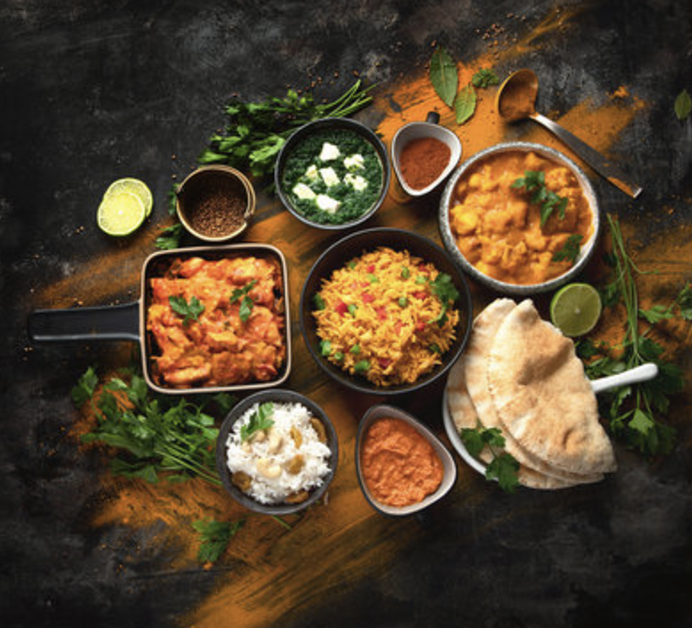
\includegraphics[width=0.7\textwidth]{all_food.png} 
    \vfill
    {\large \today\par}
\end{titlepage}

% Contents
\tableofcontents
\begin{enumerate}
    \item Butter Chicken
    \item Masala Dosa
    \item Paneer Butter Masala
    \item Aloo Gobi
\end{enumerate}
\newpage

% Butter Chicken
\section*{Butter Chicken (Murgh Makhani)}
\textbf{Ingredients:}
\begin{itemize}
    \item 500g chicken (boneless, diced)
    \item 1 cup yogurt
    \item 2 tbsp ginger-garlic paste
    \item 2 tbsp butter
    \item 1 cup tomato puree
    \item 1/2 cup cream
    \item Spices: garam masala, turmeric, red chili powder, salt, and kasuri methi
\end{itemize}

\textbf{Instructions:}
\begin{enumerate}
    \item Marinate the chicken in yogurt, ginger-garlic paste, and spices for 1 hour.
    \item Cook the marinated chicken until tender.
    \item In a pan, melt butter, add tomato puree, and cook with spices.
    \item Add the cooked chicken and cream; simmer for 10 minutes.
    \item Garnish with kasuri methi and serve with naan or rice.
\end{enumerate}

\textbf{Cooking Time:} 1 hour \\
\textbf{Servings:} 4
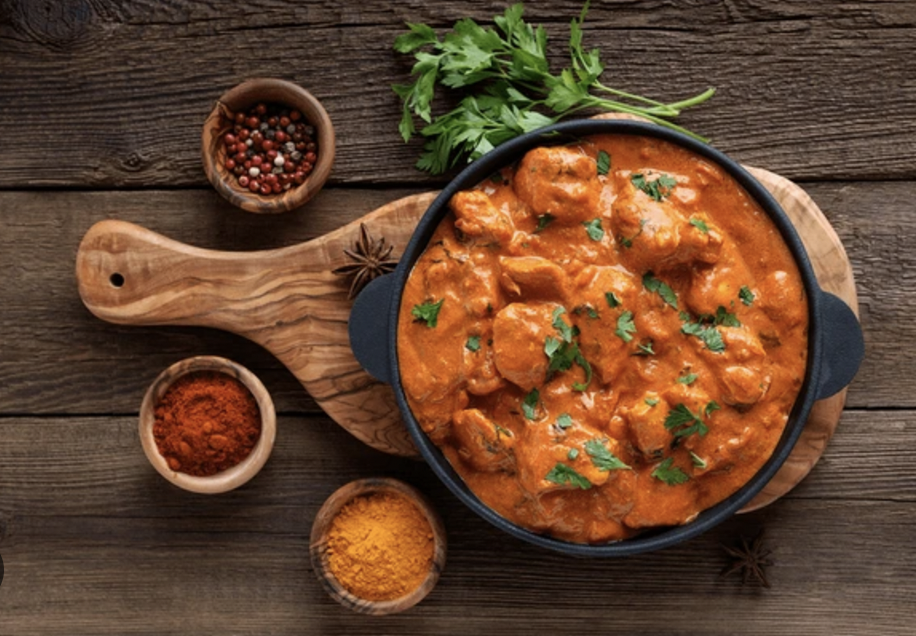
\includegraphics[width=0.7\textwidth]{butter_chicken.png} 
\newpage

%Masala Dosa
\section*{Masala Dosa}
\textbf{Ingredients:}
\begin{itemize}
    \item 2 cups dosa batter
    \item 2 boiled potatoes (mashed)
    \item 1 onion (sliced)
    \item Spices: mustard seeds, curry leaves, turmeric, and green chilies
    \item Ghee or oil for cooking
\end{itemize}

\textbf{Instructions:}
\begin{enumerate}
    \item Heat oil, add mustard seeds, curry leaves, and onions. Sauté until golden.
    \item Add turmeric, green chilies, and mashed potatoes; mix well.
    \item Spread dosa batter on a hot pan, cook until crispy, and add the potato filling.
    \item Fold the dosa and serve hot with coconut chutney and sambhar.
\end{enumerate}

\textbf{Cooking Time:} 45 minutes \\
\textbf{Servings:} 3
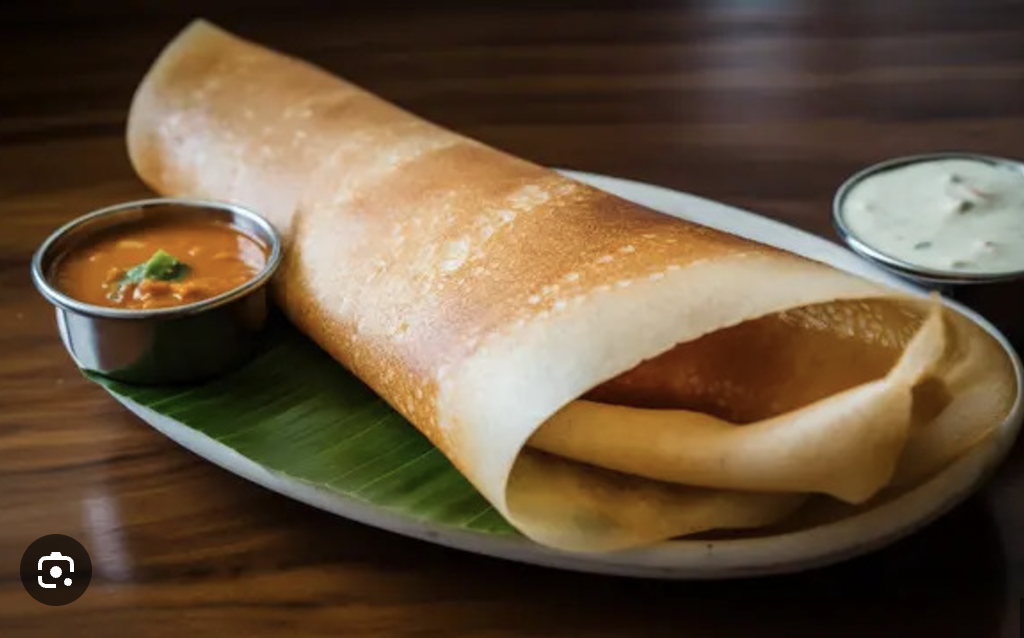
\includegraphics[width=0.7\textwidth]{masala_dosa.png} 
\newpage

% Paneer Butter Masala
\section*{Paneer Butter Masala}
\textbf{Ingredients:}
\begin{itemize}
    \item 250g paneer (cubed)
    \item 2 onions (pureed)
    \item 3 tomatoes (pureed)
    \item 2 tbsp butter
    \item 1/2 cup cream
    \item Spices: garam masala, red chili powder, turmeric, kasuri methi, and salt
\end{itemize}

\textbf{Instructions:}
\begin{enumerate}
    \item Heat butter in a pan, add onion puree, and sauté until golden.
    \item Add tomato puree and spices; cook until the oil separates.
    \item Add paneer cubes and cream; simmer for 5-10 minutes.
    \item Garnish with kasuri methi and serve with naan or roti.
\end{enumerate}

\textbf{Cooking Time:} 30 minutes \\
\textbf{Servings:} 4
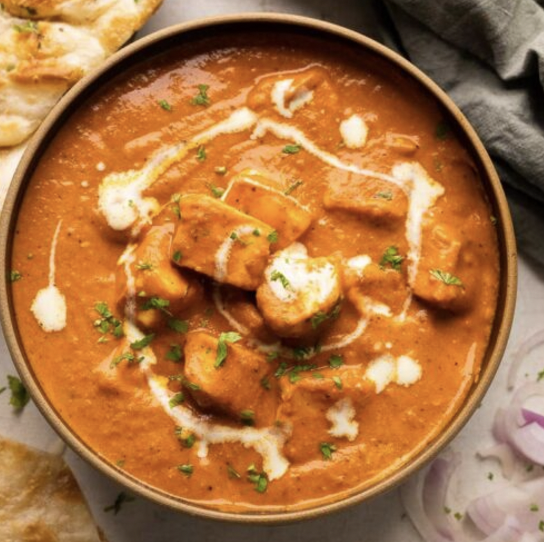
\includegraphics[width=0.7\textwidth]{paneer_butter_masala.png} 
\newpage

% Aloo Gobi
\section*{Aloo Gobi}
\textbf{Ingredients:}
\begin{itemize}
    \item 2 potatoes (cubed)
    \item 1 small cauliflower (florets)
    \item 1 onion (chopped)
    \item 2 tomatoes (chopped)
    \item Spices: cumin seeds, turmeric, garam masala, red chili powder, and salt
    \item Fresh coriander for garnish
\end{itemize}

\textbf{Instructions:}
\begin{enumerate}
    \item Heat oil in a pan, add cumin seeds, and sauté onions until golden.
    \item Add tomatoes and spices; cook until the oil separates.
    \item Add potatoes and cauliflower; mix well and cover with a lid.
    \item Cook on low heat until the vegetables are tender.
    \item Garnish with fresh coriander and serve with paratha or rice.
\end{enumerate}

\textbf{Cooking Time:} 40 minutes \\
\textbf{Servings:} 4
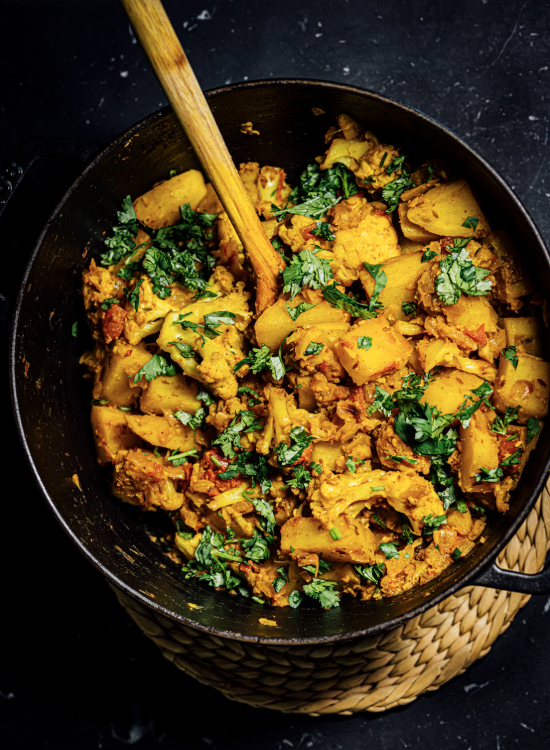
\includegraphics[width=0.7\textwidth]{aloo_gobi.png} 
\newpage


\begin{multicols}{2}
\section*{Cooking Tips}
\begin{itemize}
    \item Use fresh spices for maximum flavor.
    \item Roast dry spices before grinding for richer masalas.
    \item Always taste and adjust salt/spices at the end.
    \item Use ghee for a richer taste in Indian curries.
\end{itemize}
\end{multicols}

\end{document}
